\documentclass[UTF8]{ctexart}
\usepackage{fancyhdr}
\pagestyle{empty}
\usepackage{geometry}
\geometry{top=1cm,right=1cm,left=1cm}
\geometry{paperwidth=18cm,paperheight=28cm}
\usepackage[pdftex, hidelinks]{hyperref}
\usepackage{color}
\usepackage{fontawesome}
\usepackage{graphicx}

\begin{document}
%%%%%%%%%%%%%%%%%%%%%%%%%%%%%%%%%%%
\begin{flushleft}
\Huge \textbf{卢意}\\
\vspace{-50pt}
\begin{table}[h]
\begin{tabular*}{1\textwidth}{l@{\extracolsep{\fill}}l}
{}&{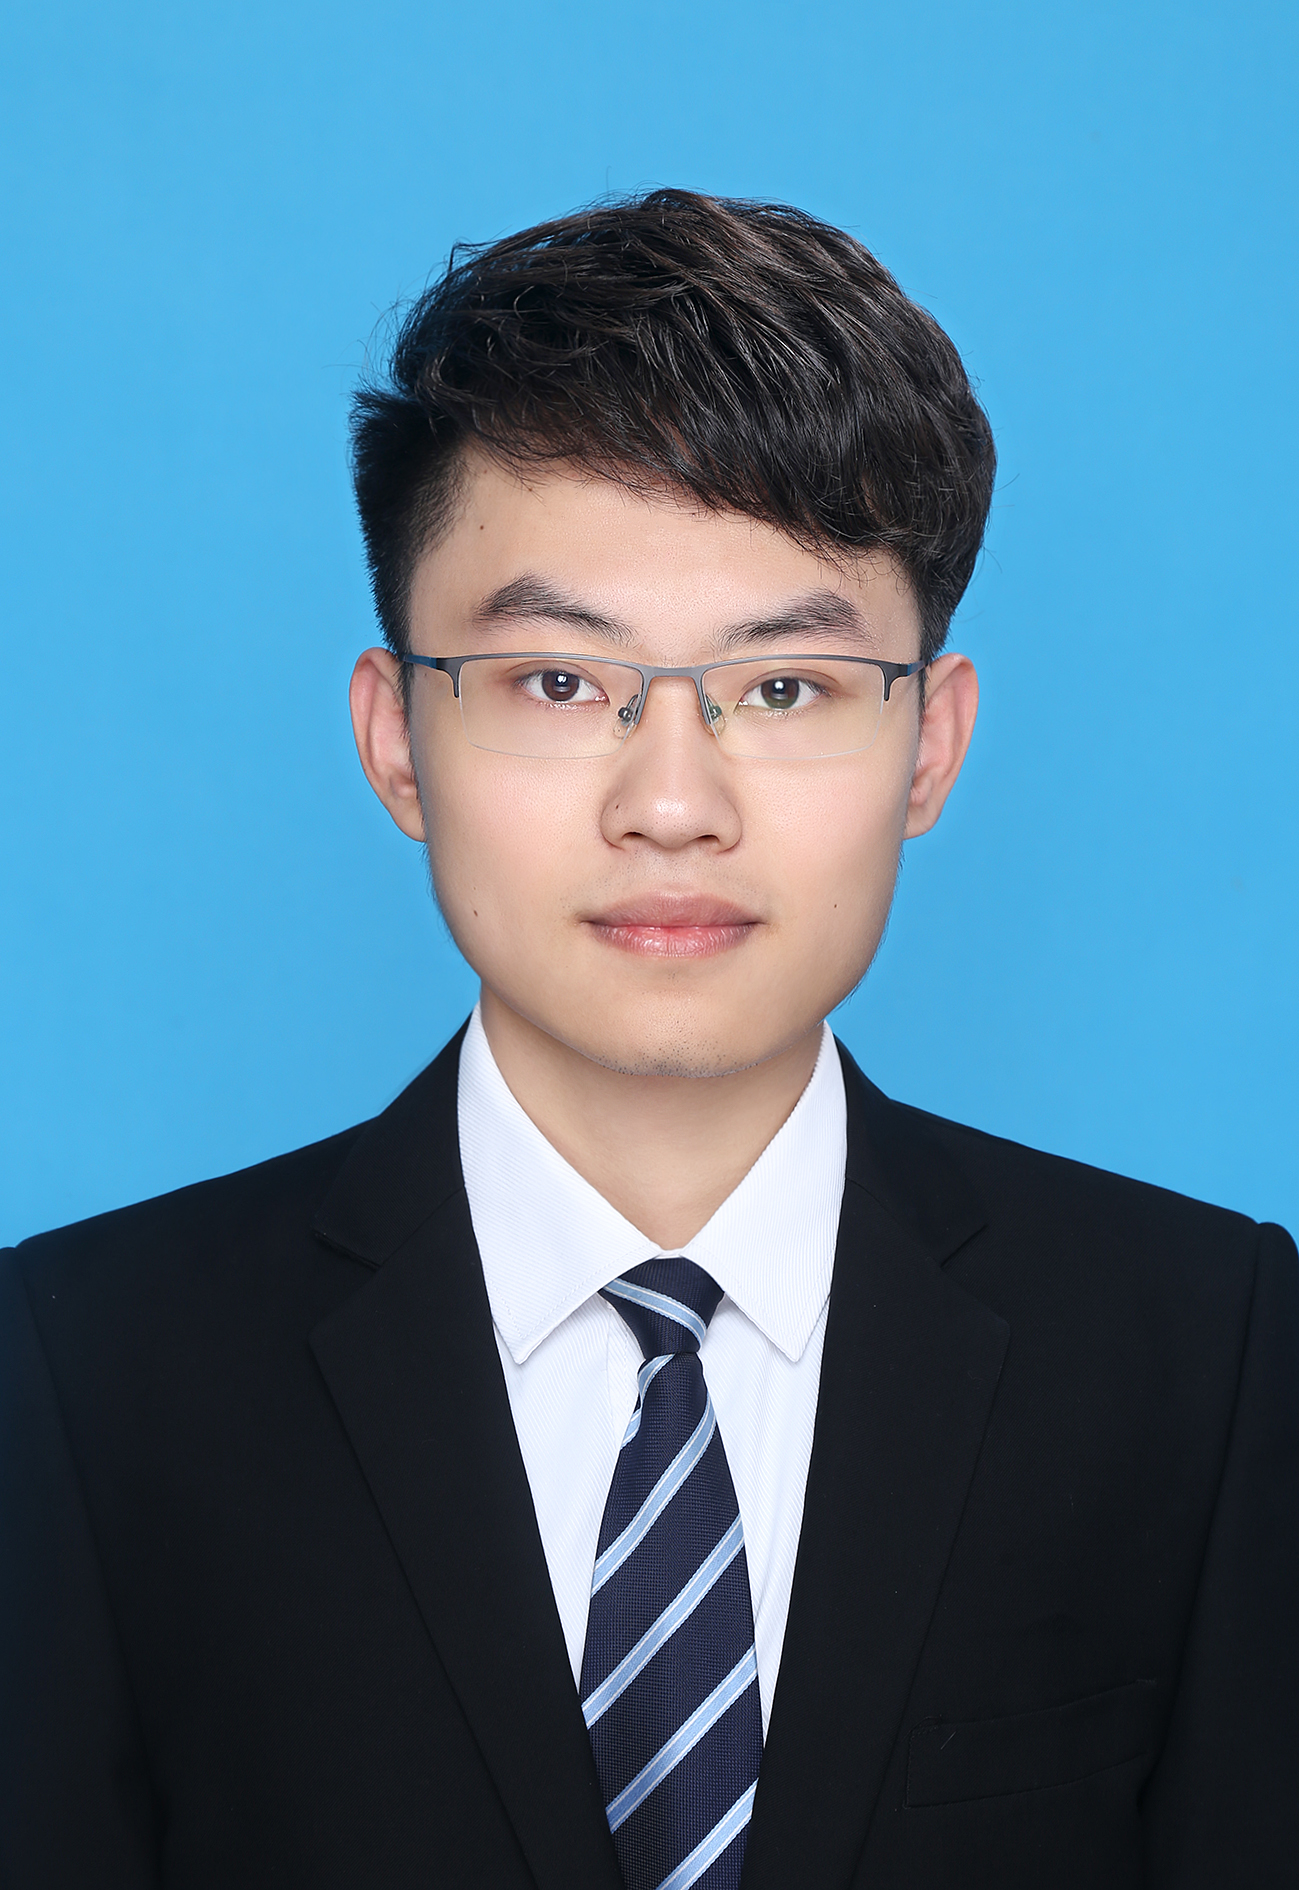
\includegraphics[scale=0.8]{Luyi.JPG}}
\end{tabular*}
\end{table}
\vspace{-80pt}
\normalsize 意向学习方向:IC设计$\vert$FPGA开发\\
\normalsize 出生年月:2000年2月$\vert$性别:男\\
\faEnvelope:{\color{blue}{\underline{baymax.ly@whut.edu.cn}}}$\vert$
\faMobilePhone:18370752330\\
\faMapMarker:湖北省武汉市洪山区武汉理工大学鉴湖校区$\vert$430070
\end{flushleft}
%%%%%%%%%%%%%%%%%%%%%%%%%%%%%%%%%%%
%          教育背景
%%%%%%%%%%%%%%%%%%%%%%%%%%%%%%%%%%%
\noindent\faGraduationCap\quad 教育背景\\
\rule[12pt]{16cm}{0.005em}\\[-12pt]
\textbf{武汉理工大学}$\vert$信息工程学院$\vert$电子科学与技术系$\vert$本科在读
\hspace{3em} \textbf{2018年9月$\sim$2022年6月} \\
\textbf{主修课程:}\quad {模拟电子技术基础(94),数字电子技术基础(97),半导体物理基础(90)}\\
{\textbf{GPA}:3.701/5.0,}{\textbf{专业排名}:11/118,}{\textbf{英语水平}:CET4/479}\\[-10pt]

%%%%%%%%%%%%%%%%%%%%%%%%%%%%%%%%%%%
%          专业技能
%%%%%%%%%%%%%%%%%%%%%%%%%%%%%%%%%%%
\noindent\faGears\quad 专业技能\\
\rule[12pt]{16cm}{0.005em}\\[-12pt]
\textbf{开发平台:}\hspace{1em} Win10\hspace{1em}Ubuntu 18.04.\\
\textbf{开发语言:}\hspace{1em} C\hspace{1em}C++\hspace{1em}Verilog HDL.\\
\textbf{开发软件:}\hspace{1em} MDK\hspace{1em}Vivado\hspace{1em}Vivado HLS\hspace{1em}Altium Designer...\\[-10pt]

%%%%%%%%%%%%%%%%%%%%%%%%%%%%%%%%%%%
%          所获荣誉
%%%%%%%%%%%%%%%%%%%%%%%%%%%%%%%%%%%
\noindent\faTrophy\quad 所获奖项\\
\rule[12pt]{16cm}{0.005em}\\[-12pt]
\textbf{2019.11}\quad 武汉理工大学院三好学生\\
\textbf{2019.12}\quad 武汉理工大学第十九届创新杯大学生课外学术作品竞赛$\vert$校一等奖$\vert$排位1\\
\textbf{2020.09}\quad 武汉理工大学优秀社团会长|2021年带领电子科技协会冲上五星级,创历史新高\\
\textbf{2020.10}\quad 2020年湖北省大学生电子设计“TI杯”竞赛$\vert$三等奖$\vert$排位1\\
\textbf{2020.11}\quad “翼展时代奖学金”\\
\textbf{2020.12}\quad 第四届全国大学生FPGA创新设计竞赛决赛$\vert$二等奖$\vert$排位1\\
\textbf{2021.06}\quad 第五届集成电路创新创业大赛校赛$\vert$二等奖并入围华中赛区决赛$\vert$排位1\\
\textbf{2021.07}\quad 武汉理工大学第十四届电工电子创新设计大赛$\vert$一等奖并推荐2021全国电赛$\vert$排位1\\[-10pt]

\noindent\faLeanpub\quad 论文专利\\
\rule[12pt]{16cm}{0.005em}\\[-12pt]
$>[1]${Lu, Y., Zhang, X F., & Ai, Q S. (2021).} Mechanism Design and Analysis of a Multi-DOF Flexible 
Ankle Rehabilitation Robot.Journal of Physics: Conference Series 2021 International Conference
 on Intelligent Manufacturing and Industrial Automation, CIMIA 2021, March 26, 2021 - March 28, 
 2021, Guilin, China.\hspace{16em}    \textbf{EI Accession number:}20211910341978\\[-10pt]

%%%%%%%%%%%%%%%%%%%%%%%%%%%%%%%%%%%
%          社会实践
%%%%%%%%%%%%%%%%%%%%%%%%%%%%%%%%%%%

\noindent\faWrench\quad 项目经历\\
\rule[12pt]{16cm}{0.005em}\\[-12pt]
\textbf{2020.4——2021.5}\quad 主持国家级创新训练项目《一种多自由度柔性脚踝康复机器人》,项目编号:
202010497086,指导老师:艾青松老师。期间主要主要负责根据指导老师的研究算法搭建Labview控制系统。
期间分别以第一作者、第二作者发表EI会议论文各一篇。\\[10pt]
\textbf{2021.4至今}\quad 依托第五届集成电路创新创业大赛申报校级创新训练项目《基于FPGA开源软核处
理器Cortex-M3的硬件加速系统》,项目编号:2021-XX-B1-06。截止到6月初,完成了基于侦差法的运动目标检
测系统,并入围华中赛区决赛。截止到2021年7月初,已经完成基于ZYBO-Z7和YOLOv2的图像分类系统,通过HLS
优化并设计了YOLOv2硬件加速器,作为决赛参赛作品。\\
\end{document}